\begin{figure}[H]
\centering
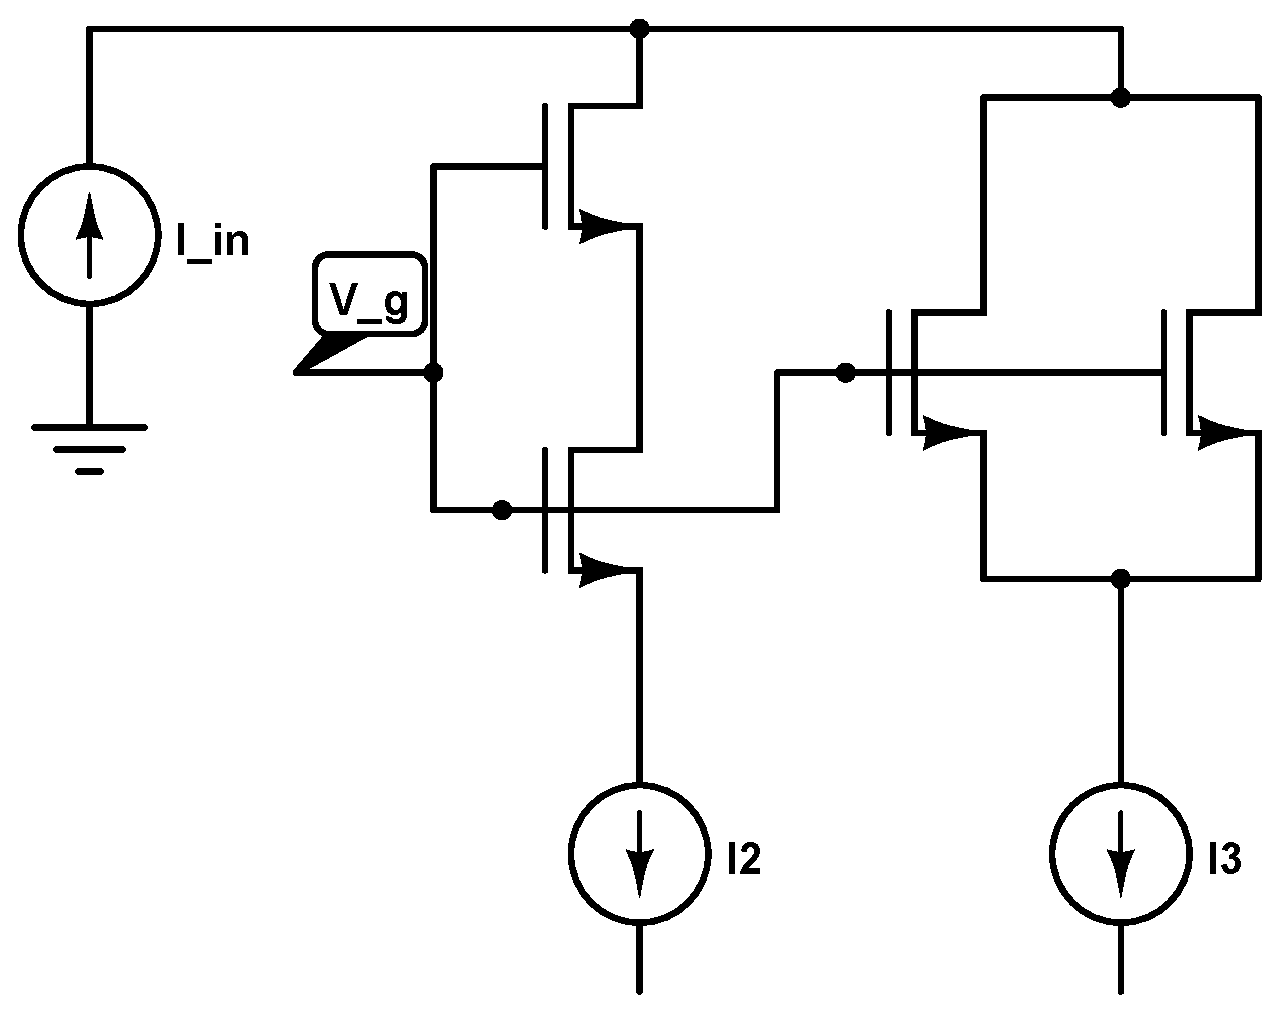
\includegraphics[width=0.55\linewidth]{../Figures/Experiment3CircuitDiagram2.eps}
\caption{A diagram of the circuit used in Experiment 3 Section 2}
\label{fig:exp3circuit2}
\end{figure}


Next, we constructed the two-way current divider shown in Figure \ref{fig:exp3circuit2}, such that the divider ratio was
a small integer multiple. We measured the output current as we swept the input current, fitting a straight line to the data collected.

\begin{figure}[H]
\centering
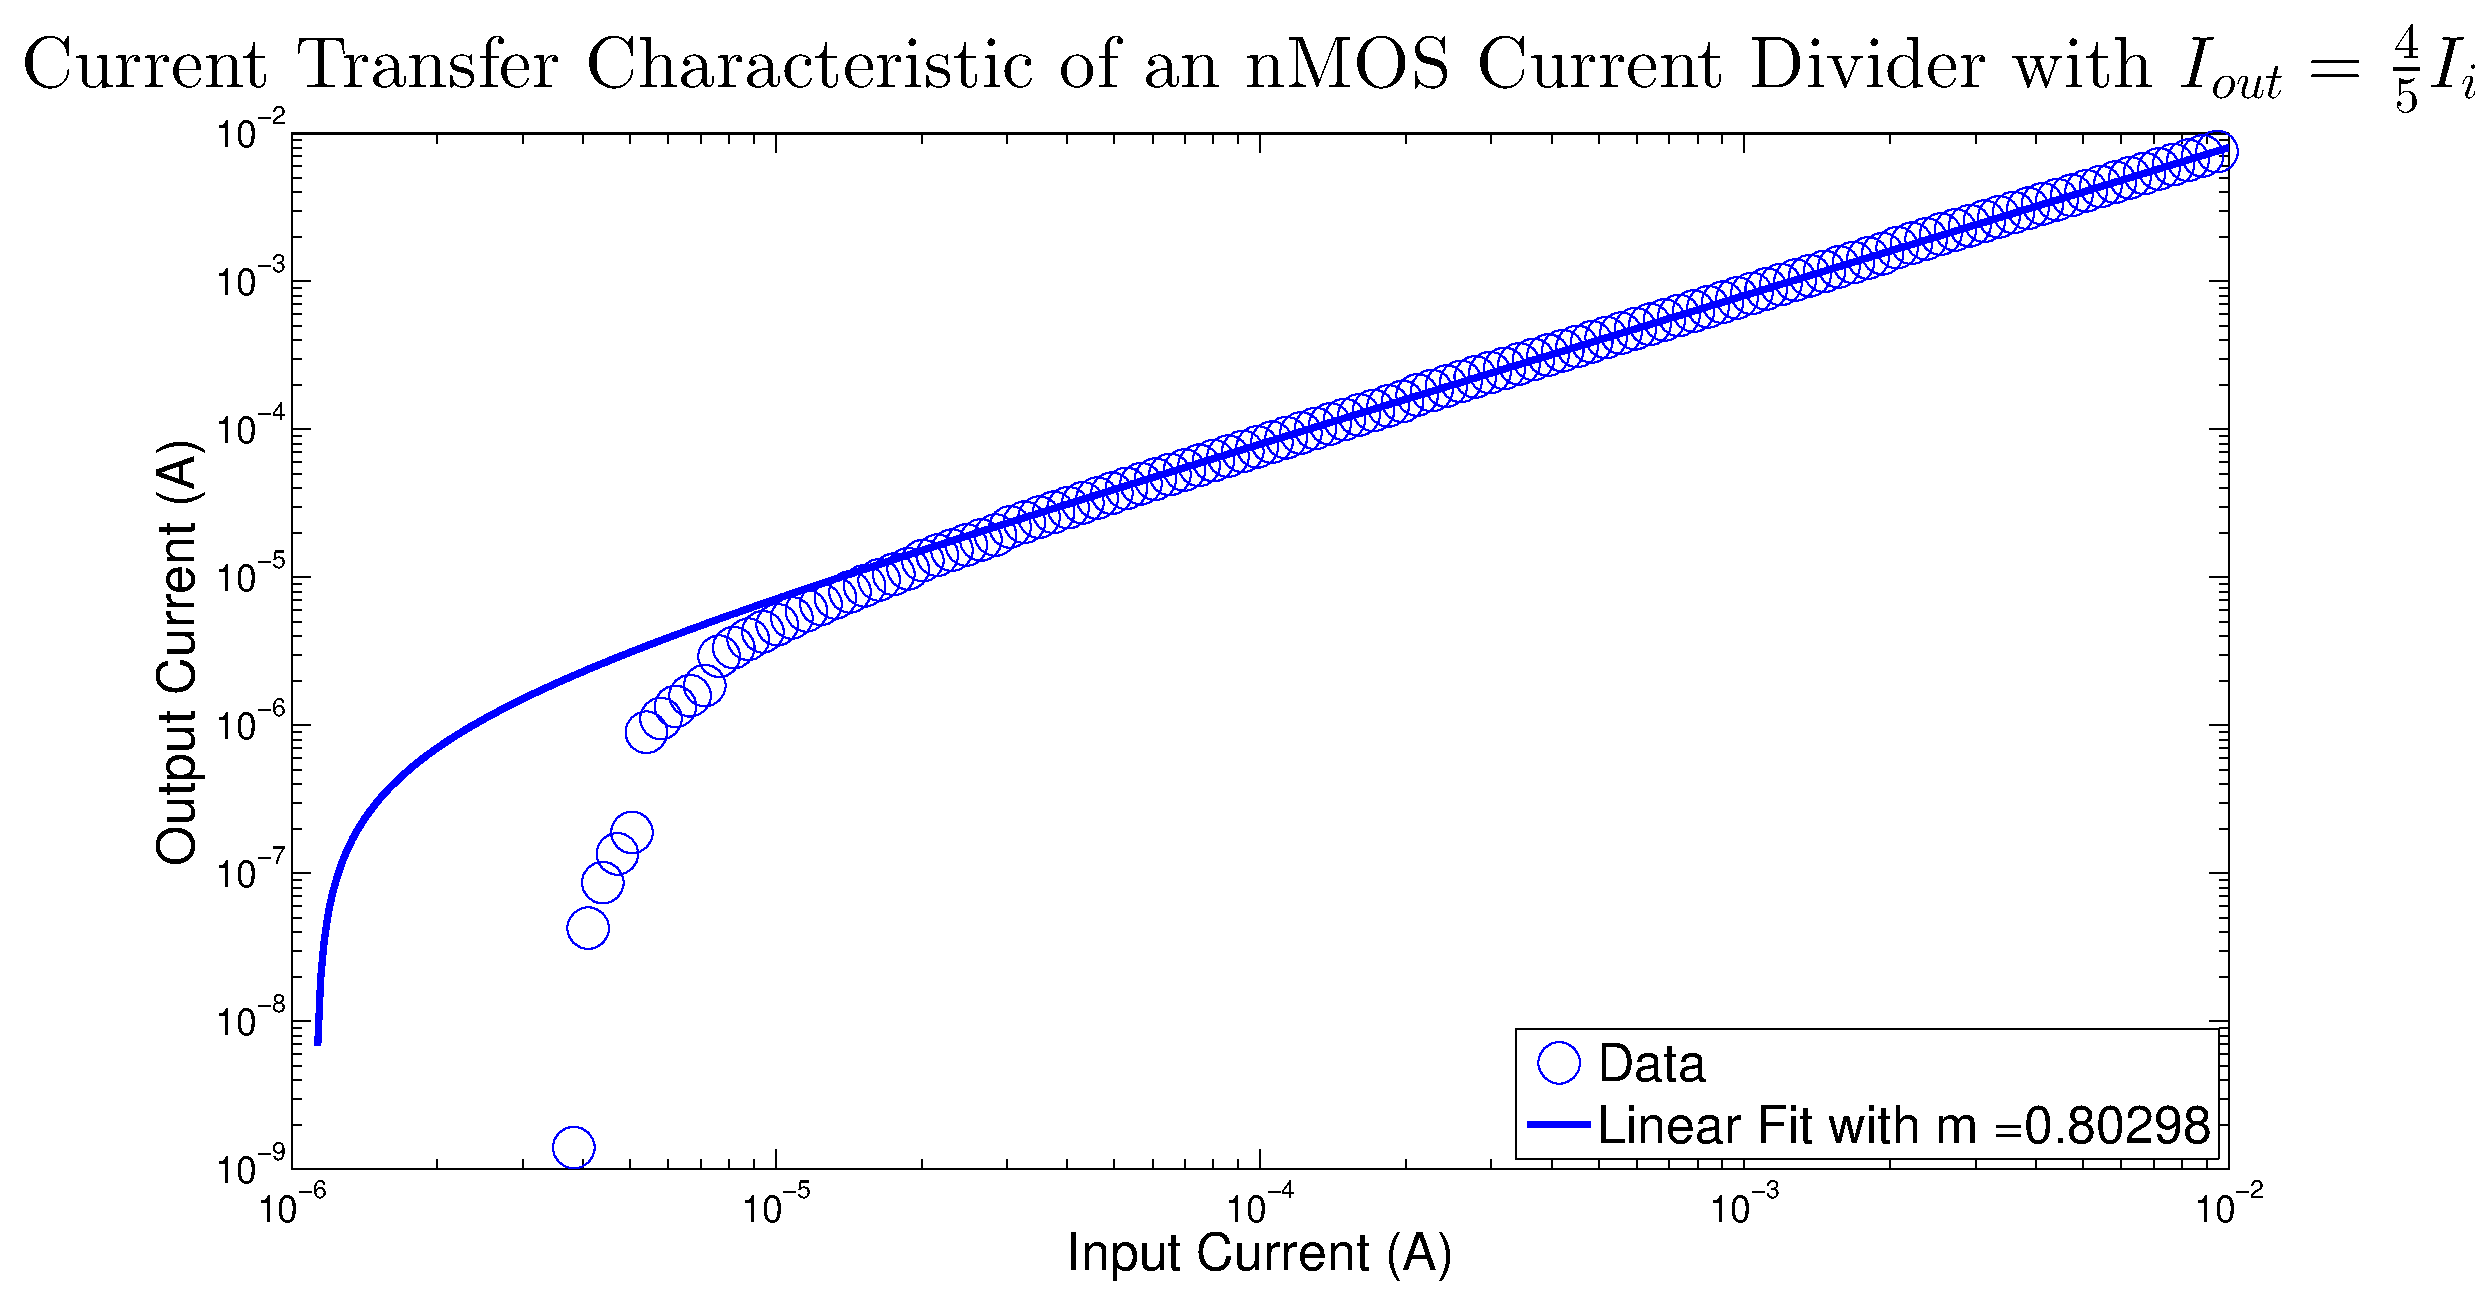
\includegraphics[width=\linewidth]{../Figures/Experiment3Figure2.eps}
\caption{A plot of the current through the parallel combinaton of \nMOS, as a function of input current.}
\label{fig:exp3fit2}
\end{figure}
As can be seen in Figure \ref{fig:exp3fit2}, the data fit a straight line well, with an extracted slope of $0.80298$. Drawing upon our previous knowledge from Experiment 2, where we found that the series combination of two \nMOS transistors passed half the current as a single \nMOS, and the parallel combination passed twice the current of a single \nMOS, we can infer that the series combination passed one quarter the current of a parallel combination. 
Thus, for a given set of voltages, \Vg, \Vd, \Vb, \Vd and \Vs, we expect the theoretical ratio of current passed to be 1:4 between the series and parallel combinations, respectively. A 1:4 ratio is the same as a fifth of the current being passed through the series combination, and four-fifths of the current through the parallel combination. As seen in Figure \ref{fig:exp3fit2}, the extract slope was almost exactly $4/5$ or $0.8$.

